% ltex: language=it
\chapter{Introduzione}\label{chap:introduzione} % (fold)
\begin{definition}{Intelligenza}{int}
    Complesso di facoltà psichiche e mentali che consentono all'uomo di pensare, comprendere o spiegare i fatti o le azioni, elaborare modelli astratti della realtà, intendere e farsi intendere dagli altri, giudicare e lo rendono insieme capace di adattarsi a situazioni nuove e di modificare la situazione stessa quando questa presenta ostacoli all'adattamento.
\end{definition}
\begin{definition}{Intelligenza Artificiale}{ia}
    Riproduzione parziale dell'attività intellettuale propria dell'uomo (con particolare riguardo ai processi di apprendimento, di riconoscimento, di scelta) realizzata o attraverso l'elaborazione di modelli ideali, o, concretamente, con la messa a punto di macchine che utilizzano per lo più a tale fine elaboratori elettronici.
\end{definition}
%
\section{Ragionamento}\label{sub:ragionamento} % (fold)
\begin{definition}{Deduttivo}{}
    \textbf{Aristotele}, nel ragionamento deduttivo, o sillogismo, la verità delle premesse garantisce la verità della conclusione.
    \[
        \begin{matrix}
            \text{REGOLA } \pt{C \to R}: \text{ Tutti gli uomini sono mortali} \\
            \text{CASO } \pt{C_1}: \text{ Socrate è un uomo} \\
            \textit{quindi} \\
            \text{RISULTATO } \pt{R_1}: \text{ Socrate è mortale} \\
        \end{matrix}
    \]
\end{definition}
Il ragionamento deduttivo è il fondamento di gran parte delle dimostrazioni e teoremi della matematica, ma non ci permette di scoprire o prevedere fatti nuovi e quindi di ampliare le nostre conoscenze, compiendo un `salto' dal noto all'ignoto.
\begin{definition}{Induttivo}{}
    Nel ragionamento induttivo, diversamente da quello deduttivo, le premesse (caso/i particolare/i) forniscono un'evidenza più o meno forte a sostegno della conclusione (generalizzazione), ma non ne garantiscono necessariamente la verità.
\end{definition}
I ragionamenti induttivi comportano quindi un rischio da cui sono esenti quelli deduttivi: possono portare da premesse vere a conclusioni false.
Il ragionamento induttivo è quindi un ragionamento \textbf{probabilistico}, le cui conclusioni dipendono dal grado di probabilità delle informazioni contenute nelle premesse.
\[
    \begin{matrix}
        \text{CASO } \pt{C_1}: \text{ Socrate era un uomo} \\
        \text{RISULTATO } \pt{R_1}: \text{ Socrate morì} \\
        \textit{quindi} \\
        \text{REGOLA } \pt{C \to R}: \text{ Tutti gli uomini sono mortali} \\
    \end{matrix}
\]
La forma più comune di ragionamento induttivo è la \textbf{generalizzazione}, con cui otteniamo informazioni su un gruppo di cose, persone, eventi, oggetti e così via, esaminando una porzione --- o campione --- di quel gruppo.
\emptyln{}
Una forma di <<induzione molto potente>> è il ragionamento per \textbf{Analogia}, che consiste con qualcos'altro.
Questo permette agli esseri umani di:
\begin{itemize}
    \item utilizzare metafore;
    \item astrarre concetti <<portandoli>> da un domino all'altro;
    \item essere creativi;
\end{itemize}
\begin{definition}{Abduttivo}{}
    Il ragionamento è probabilistico, ma invece di generalizzare ci si muove \textit{lateralmente}, ipotizzando che un'implicazione valga anche al contrario.
\[
    \begin{matrix}
        \text{REGOLA } \pt{C \to R}: \text{ Tutti gli uomini sono mortali} \\
        \text{RISULTATO } \pt{R_1}: \text{ Socrate morì} \\
        \textit{quindi} \\
        \text{CASO } \pt{C_1}: \text{ Socrate era un uomo} \\
    \end{matrix}
\]
\textit{induzione per scienziati, l'abduzione per investigatori\ldots}
\end{definition}
%
% section Ragionamento (end)
\section{Intelligenza Artificiale e Machine Learning}\label{sub:intelligenza_artificiale_e_machine_learning} % (fold)
L'\ac{ia} è una disciplina molto vasta che copre diverse tematiche, tra cui:
\begin{itemize}
    \item Problem Solving:
    \begin{itemize}
        \item Search algorithms;
        \item Adversarial Search and Games;
        \item Constraint Satisfaction Problems;
    \end{itemize}
    \item Knowledge, Reasoning and Planning:
    \begin{itemize}
        \item First Order Logic, Inference;
        \item Prolog;
    \end{itemize}
    \item Uncertain Knowledge:
    \begin{itemize}
        \item Probabilistic Reasoning;
        \item Bayesian Network;
    \end{itemize}
    \item Multi-Agents;
    \item Machine Learning:
    \begin{itemize}
        \item Classificazione, Regressione, Clustering;
        \item Neural networks and Deep Learning;
        \item Generative AI and Large Language Models;
    \end{itemize}
\end{itemize}
%
% section Intelligenza Artificiale e Machine Learning (end)
\section{Machine Learning}\label{sub:machine_learning} % (fold)
Un modello di Machine Learning (apprendimento automatico) durante la fase di training apprende a partire da esempi.
Successivamente è in grado id generalizzare e gestire nuovi dati nello stesso dominio applicativo.
Più formalmente: ``impara dagli esempi a migliorare le proprie prestazioni per la gestione di nuovi dati provenienti dalla stessa sorgente''.
\begin{cimage}
    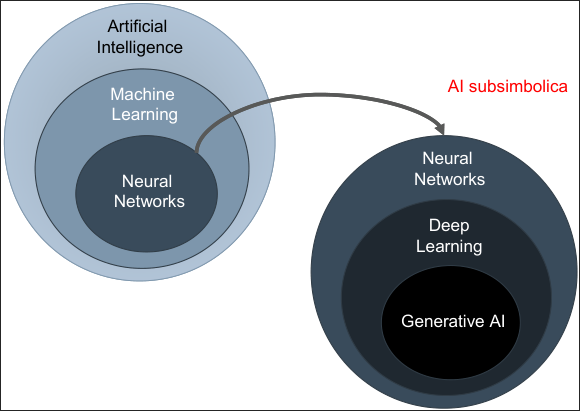
\includegraphics[width=.6\textwidth]{assets/ai-simbolica.png}
    \caption{AI sub-simbolica}\label{fig:ai-sub-simbol}
\end{cimage}
Il machine learning è oggi l'approccio più importante nell'ambito dell'intelligenza artificiale.
L'apprendimento è una componente chiave del ragionamento; inoltre permette di gestire la complessità di applicazioni reali, talvolta troppo complesse per poter essere modellate efficacemente.
Apprendere il comportamento desiderato dai dati/esempi forniti, semplifica lo sviluppo di applicazioni; rende possibile esplorare/comprendere i dati (mining) senza la necessità di programmazione esplicita.
% section Machine Learning (end)
\section{Intelligenza artificiale e ``forza bruta''}\label{sub:intelligenza_artificiale_e_forza_bruta_} % (fold)
\begin{definition}{Brute-Force}{brute-force}
    In alcuni domini applicativi un calcolatore è in grado di risolvere problemi in modo ottimo semplicemente enumerando e valutando tutte le possibili alternative.
\end{definition}
\\
Nella maggior parte dei casi però la valutazione esaustiva di tutte le possibili soluzioni non è computazionalmente gestibile, e si usano tecniche di ricerca che utilizzano \textbf{euristici} (più o meno intelligenti) per ridurre il numero di casi da valutare.
\\
Talvolta si utilizza il termine \textbf{Weak AI} per caratterizzare sistemi capaci di risolvere problemi complessi senza però capacità di ragionamento e comprensione.
Una particolare famiglia di algoritmi denominata \textbf{Evolutionary Computing}, tra cui \textit{Genetic Algorithms}, è oggetto di grande interesse nell'ambito dell'Intelligenza Artificiale.
Questi algoritmi s'ispirano al principio di evoluzione degli esseri viventi.
%
% section Intelligenza artificiale e ``forza bruta'' (end)
% chapter Introduzione (end)
